\documentclass[tikz,border=6pt]{standalone}
\usetikzlibrary{arrows.meta,shapes.geometric,positioning}
\definecolor{red}{HTML}{A50F2D}\definecolor{ink}{HTML}{141414}
\definecolor{bl}{HTML}{1F5F99}\definecolor{yl}{HTML}{B07A00}\definecolor{gn}{HTML}{1B7F5F}
\tikzset{
 box/.style={draw=#1,fill=#1!12,very thick,rounded corners=3pt,align=center,minimum height=0.9cm,text=ink,inner sep=5pt},
 dec/.style={diamond,aspect=2.2,draw=#1,fill=#1!12,very thick,align=center,text=ink,inner sep=1pt},
 lab/.style={font=\sffamily\small,text=ink,fill=white,inner sep=1.5pt},
 >=Stealth}
\begin{document}
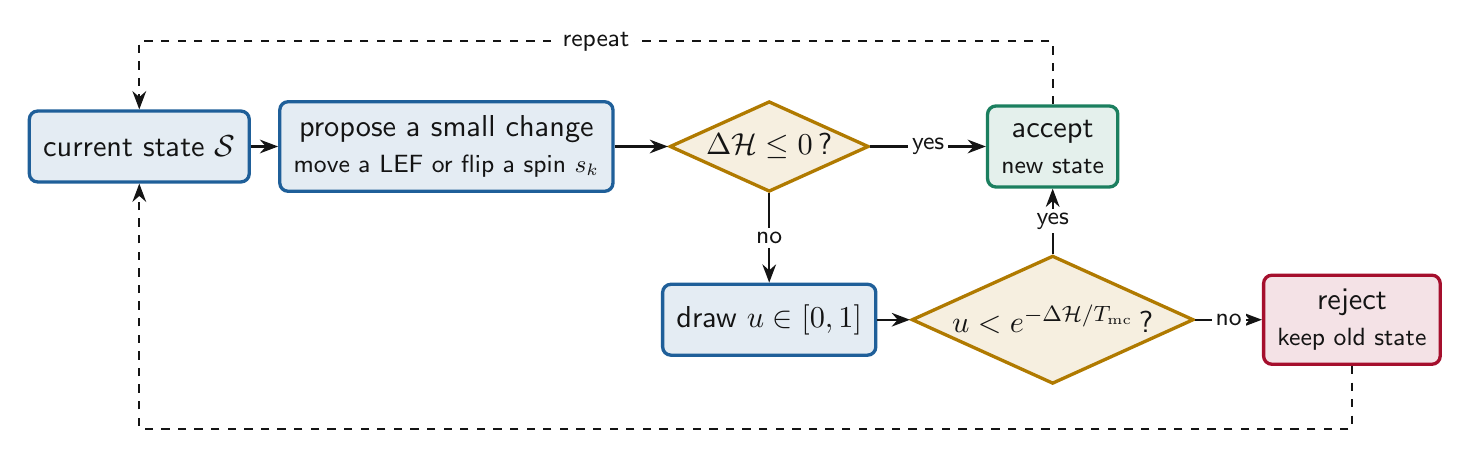
\begin{tikzpicture}[font=\sffamily\fontsize{11}{13}\selectfont]
\node[box=bl] (s) at (0,0) {current state $\mathcal{S}$};
\node[box=bl] (p) at (3.9,0) {propose a small change\\{\small move a LEF or flip a spin $s_k$}};
\node[dec=yl] (d1) at (8.0,0) {$\Delta\mathcal{H}\le 0$\,?};
\node[box=gn] (acc) at (11.6,0) {accept\\{\small new state}};
\node[box=bl] (u) at (8.0,-2.2) {draw $u\in[0,1]$};
\node[dec=yl] (d2) at (11.6,-2.2) {$u<e^{-\Delta\mathcal{H}/T_{\mathrm{mc}}}$\,?};
\node[box=red] (rej) at (15.4,-2.2) {reject\\{\small keep old state}};
\draw[->,ink,thick] (s)--(p);
\draw[->,ink,thick] (p)--(d1);
\draw[->,ink,thick] (d1)--node[lab,pos=0.5]{yes}(acc);
\draw[->,ink,thick] (d1)--node[lab,pos=0.5]{no}(u);
\draw[->,ink,thick] (u)--(d2);
\draw[->,ink,thick] (d2)--node[lab,pos=0.5]{yes}(acc);
\draw[->,ink,thick] (d2)--node[lab,pos=0.5]{no}(rej);
\draw[->,ink,thick,dashed] (acc.north) -- ++(0,0.8) -| node[lab,pos=0.25]{repeat} (s.north);
\draw[->,ink,thick,dashed] (rej.south) -- ++(0,-0.8) -| (s.south);
\end{tikzpicture}
\end{document}
